Validation of the Napali approach is intrinsically linked to validation of Makai, both with synthetic benchmarks and in-situ.
Since OPQ utilizes a custom power quality measurement device, its performance needed to be characterized prior to Makai evaluation.

\section{OPQ Box Characterization.}\label{sec:opq-box-characterization.}
A mentioned in Section~\ref{subsec:software} OPQBox generates 4 metrics in order to enable event detection.
In order to evaluate the limits of detection capabilities for each one of these metrics, an OPQBox was fed with synthetic waveform generated by the SDG1025 function generator.
By utilizing a function generator the entire device including the hardware analog front end could be evaluated.
Since the function generator is not capable of supplying $120V_{rms}$ signal, a $120mV_{rms}$ signal was fed on a low side of the OPQBox resistor divider, while the device was powered via an external 5V power supply.

\subsection{Fundamental Frequency}

Fundamental Frequency computation was evaluated by generating a 60Hz sine wave via the SDG1025 and supplying it to the OPQBox.
Calculated frequency was accumulated by analyzing the device triggering stream.
The resulting histogram is shown in Figure~\ref{fig:expdes:1}
\begin{figure}[H]
    \begin{center}
        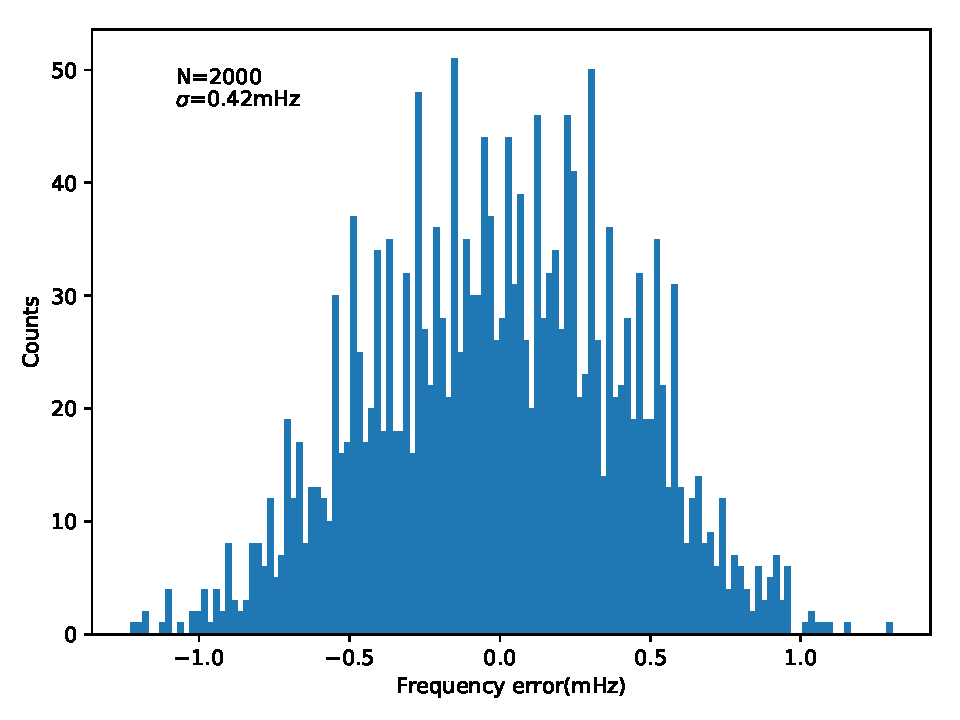
\includegraphics[width=0.6\textwidth]{img/box_eval/frequency_rms.pdf}
    \end{center}
    \caption{OPQBox frequency response.}
    \label{fig:expdes:1}
\end{figure}
As shown, the resulting distribution collected frequencies acquired over 2000s has a $\sigma=420uHz$.

\subsection{Root Mean Square Voltage}
Similarly to the fundamental frequency characterization, $V_{rms}$ calculation was evaluated by supplying the OPQBox with a 60Hz, $120mV_{rms}$ sine wave via the SDG1025.
Calculated RMS was accumulated by analyzing the device triggering stream.
The resulting histogram is shown in Figure~\ref{fig:expdes:2}

\begin{figure}[h]
    \begin{center}
        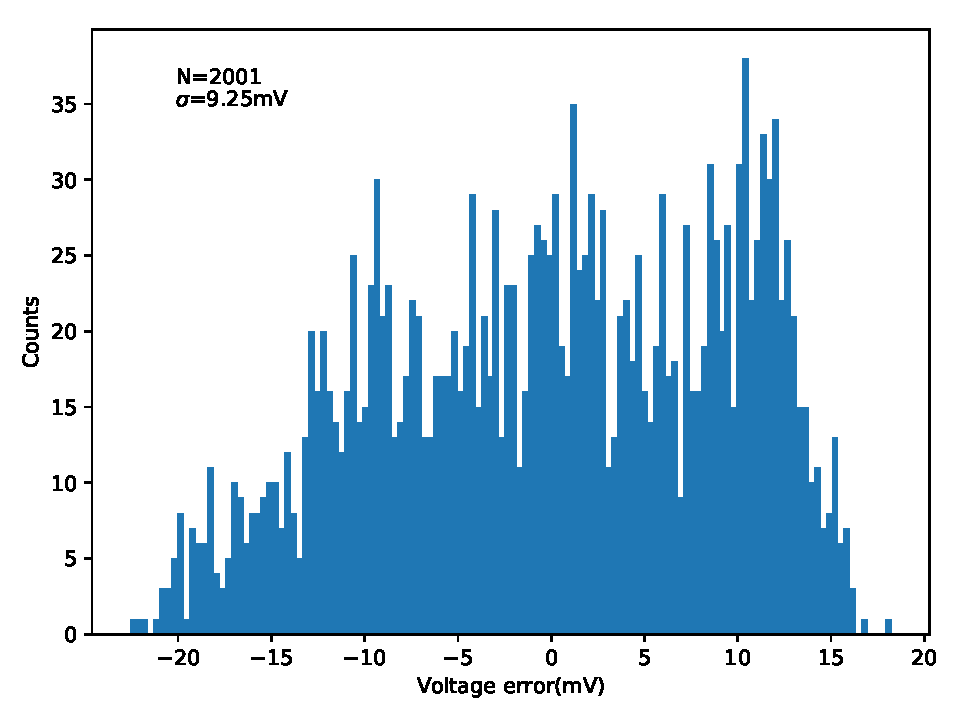
\includegraphics[width=0.6\textwidth]{img/box_eval/rms_histogram.pdf}
    \end{center}
    \caption{OPQBox $V_{rms}$ response.}
    \label{fig:expdes:2}
\end{figure}

As shown, the resulting distribution of collected $V_{rms}$ measurements, acquired over 2000s has a $\sigma=9.34mV$

\subsection{Total Harmonic Distortion}

THD performance of the OPQBox was validated by injecting a various harmonics of 60Hz superimposed onto the 60Hz, $120mV_{rms}$ sine wave into the device via the SDG1025 arbitrary waveform generation capability.
THD calculation results were acquired from the OPQBox triggering stream for analysis.
As expected resultant performance remained self-consistent across all harmonics.
Figure~\ref{fig:expdes:3} shows a histogram of the error in THD values computed form a 60Hz, $120mV_{rms}$ sinewave superimposed with a 240Hz $1.2mV_{rms}$ sine wave.
This measurement is equivalent to $1\%$ THD at the $4^{th}$ harmonic.

\begin{figure}[h]
    \begin{center}
        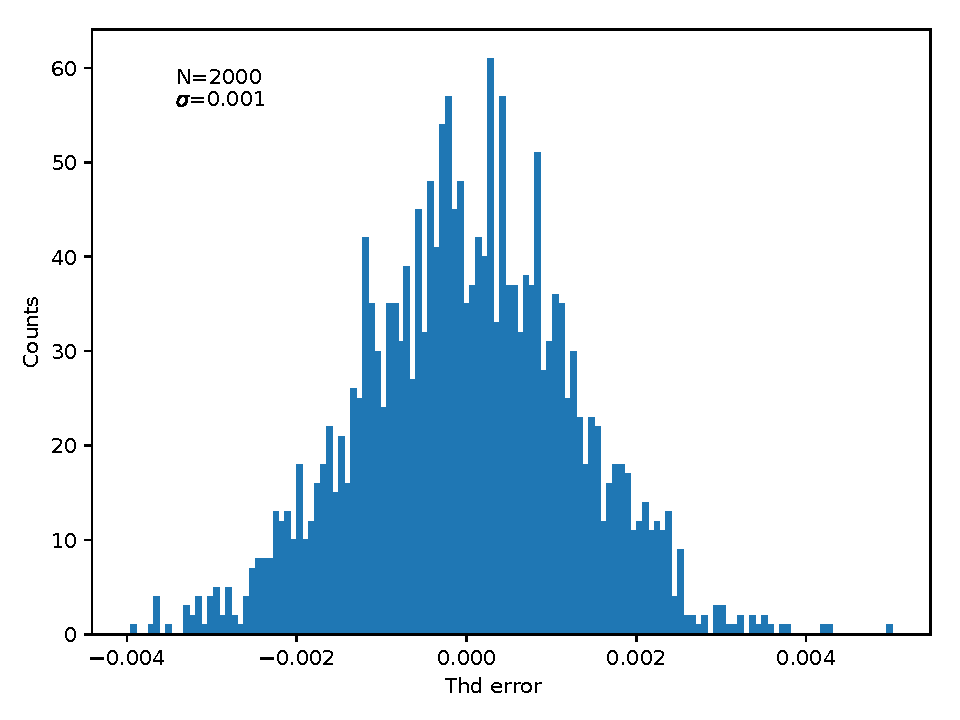
\includegraphics[width=0.6\textwidth]{img/box_eval/thd_rms.pdf}
    \end{center}
    \caption{OPQBox THD response.}
    \label{fig:expdes:3}
\end{figure}

As shown, the resulting distribution of collected THD measurements, acquired over 2000s has a $\sigma=0.001\%$.

\subsection{Transient Detection}

Transient detection performance was evaluated by injecting a transient superimposed onto the 60Hz, $120mV_{rms}$ sine wave into the device via the SDG1025 arbitrary function generation capability.
Transient detection results were acquired by capturing and analyzing the device triggering stream.
Transients of various shapes and magnitudes were tested.

\begin{figure}[h]
    \centering
    \begin{subfigure}{.5\textwidth}
        \centering
        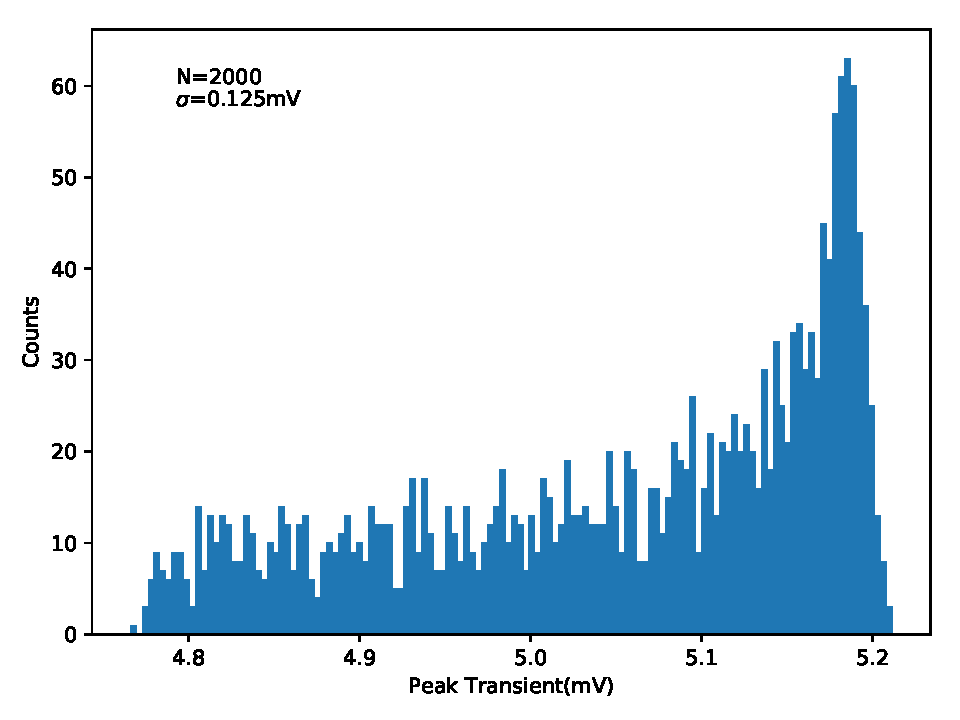
\includegraphics[width=0.9\linewidth]{img/box_eval/5v_transient_rms.pdf}
        \caption{}
        \label{fig:expdes:4:1}
    \end{subfigure}%
    \begin{subfigure}{.5\textwidth}
        \centering
        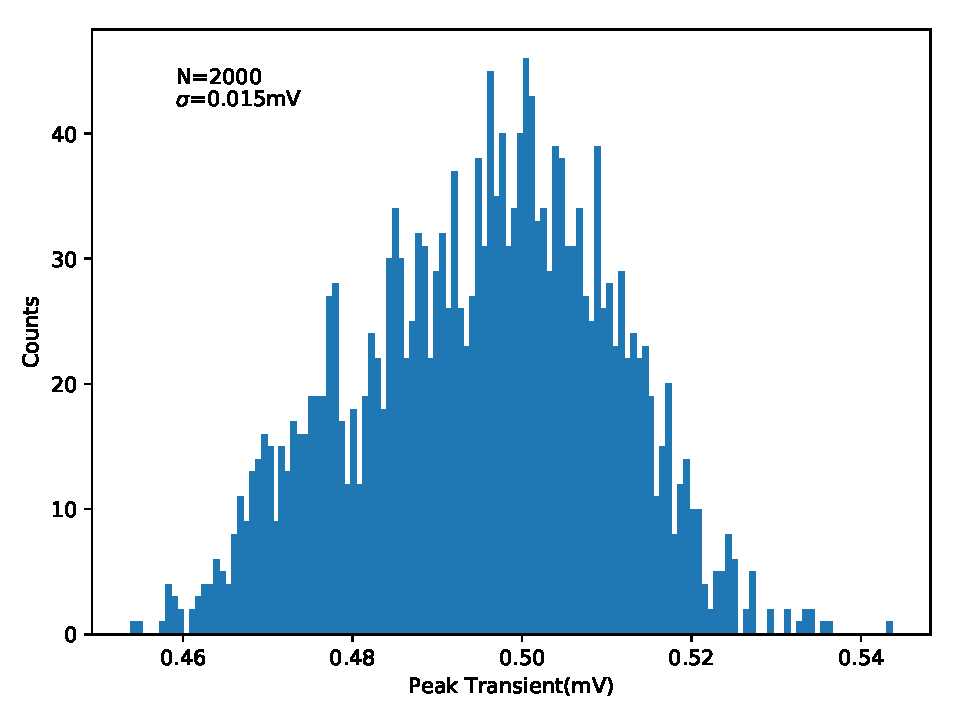
\includegraphics[width=0.9\linewidth]{img/box_eval/0p5v_transient_rms.pdf}
        \caption{}
        \label{fig:expdes:4:2}
    \end{subfigure}
    \caption{Transient detection metric with a 5V transient(a), and 0.5V transient(b)}
    \label{fig:expdes:4}
\end{figure}

Figure~\ref{fig:expdes:4} shows the resultant transient detection metric for two transients.
The shape of the transient is the same and is shown in Figure~\ref{fig:opq:8:3}.
Interestingly, in case of a 0.5V transient the metric results in a much tighter distribution with $\sigma =0.015V$, while in the case of
a 5V transient the distribution exhibits a lower sideband tail.
Since the transient is injected in a random position in the cycle, and the sampling rate of the DG1025 is significantly higher then sampling rate of the OPQBox(25Msps vs 12Ksps), the peak of the transient will sometimes fall in between the consecutive samples of the OPQBox.
In the $0.5V$ transient case this effect is alleviated, since the transient is so small.
Regardless, the result shown in Figure~\ref{fig:expdes:4:2} is presented only as a synthetic benchmark, since OPQBox is expected to operate in an environment with THD larger then $0.4\%$ at $>400Hz$ required to detect a $0.5V$ transient.
As such, the figure of $\sigma=0.125V$ should be considered valid for the OPQBox transient detection capability.
Since this metric is only used in transient detection and not characterization, it was found to be sufficient.

\section{Napali Validation}\label{sec:napali-validation.}
Napali method was validated using simulation, synthetic data with the device-in-loop, and in-situ during the deployment.
The main tunable parameter in the napali is the $\alpha$ coefficient used in the low pass filter as shown in Equation \ref{eq:iir_mean}.
This parameter determines the memory of the lowpass filter used in the calculation of the mean and the standard deviation of metrics from OPQBox data stream.
These statistics are in turn used during the Napali triggering process to locate sub-threshold gridwide events.

\subsection{Selection of $\alpha$ parameter}\label{subsec:selectrion-ofparameter}
Smaller $\alpha$ parameter corresponds to a longer memory in the low pass filter as shown in Equation \ref{eq:iir_alpha}.
This is further visualized in Figure \ref{fig:expdes:5}.
In particular this Figures \ref{fig:expdes:5:1} and \ref{fig:expdes:5:2} show the response of the IIR low pass filter to the simulated frequency measurements.
The dashed red line represents the frequency measurement, solid red line represents the filtered mean, and the blue line represents the standard diviation.
Figures \ref{fig:expdes:5:1} shows the filter response for $\alpha = 0.5$ or $T_{memory} \approx 10s $.
As evident from the plot, the mean and the standard deviation quickly recover from the transient are return to their nominal values.
Furthermore, the mean is closely tracking the random fluctuations present in the measurement.
Figures \ref{fig:expdes:5:1} shows the filter response for $\alpha = 0.05$ or $T_{memory} \approx 123s $.
While the stimuli remains the same, it takes significantly longer the statistics to recover.
Additionally, the mean no longer tracks the frequency fluctuations present in the simulated data.

\begin{figure}[h]
    \centering
    \begin{subfigure}{0.9\textwidth}
        \centering
        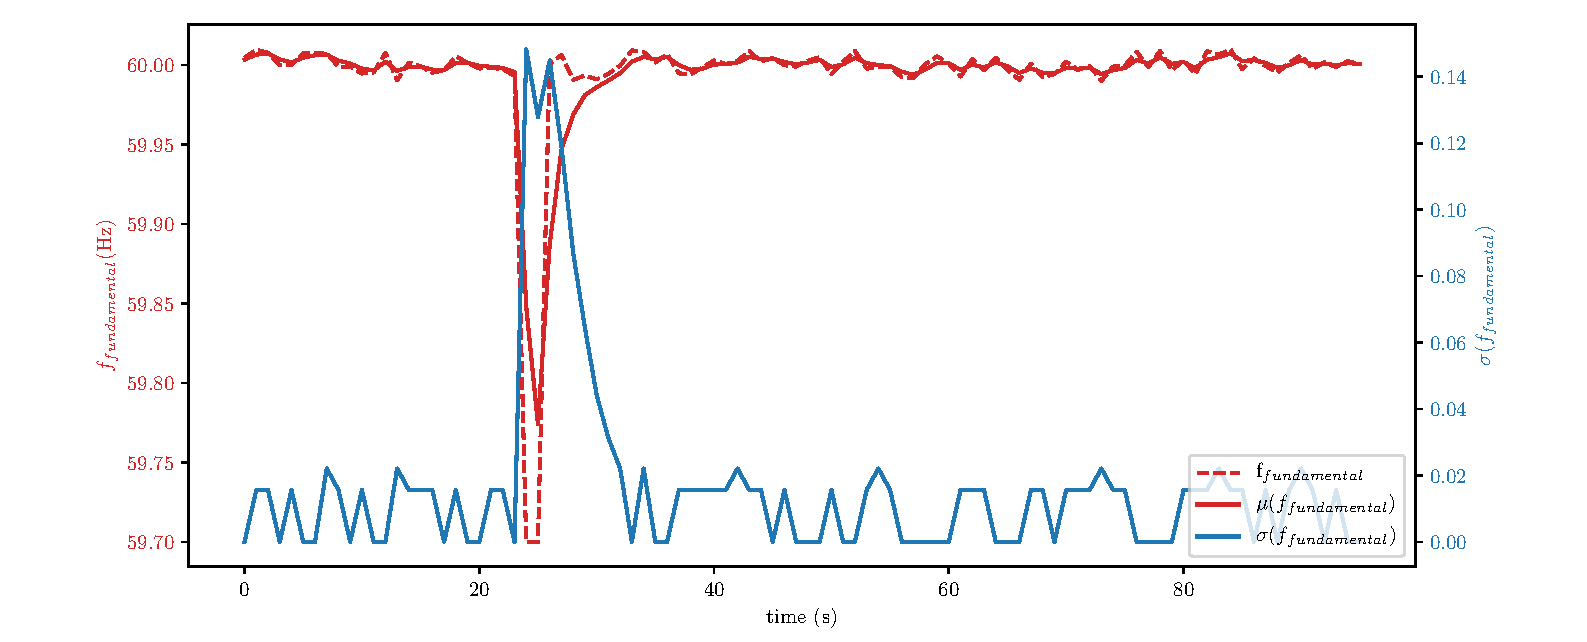
\includegraphics[width=1\linewidth]{img/napali_eval/Napali_response_freq_05.pdf}
        \caption{}
        \label{fig:expdes:5:1}
    \end{subfigure}%

    \begin{subfigure}{0.9\textwidth}
        \centering
        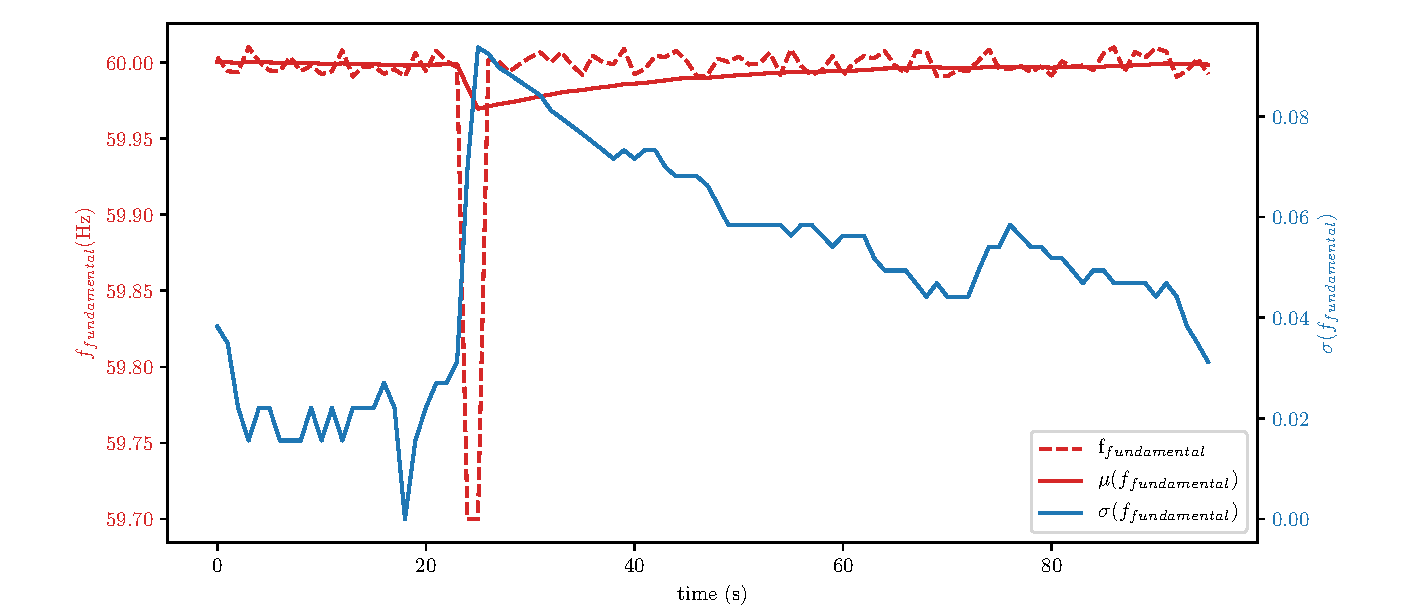
\includegraphics[width=1\linewidth]{img/napali_eval/Napali_response_freq_005.pdf}
        \caption{}
        \label{fig:expdes:5:2}
    \end{subfigure}
    \caption{$\mu$ and $\sigma$ behaviour with a)$\alpha = 0.5$ and b)$\alpha=0.05$}
    \label{fig:expdes:5}
\end{figure}

Picking the $\alpha$ parameter for Napali is extremely domain specific, as it depends on the frequency content of the triggering stream.
Intuitively, the $T_{memory}$ parameter needs to be long enough to adjust to gradual changes in the triggering stream for the mean calculation,
and dampen the standard deviation for detection of multiple consecutive anomalies.
In addition, it needs to be short enough to converge on the mean and the standard deviation during a step-like transition in the triggering stream.

Luckily, in the Power Quality domain the Napali $\alpha$ selection is fairly forgiving.
This is demonstrated in Figure \ref{fig:expdes:6}.
This graph represents the amount of time that Napali considered one of the metrics to be outside of the $3\sigma$ of the mean for various values of $\alpha$.
The triggering stream used to generate these values was captured over 24 hours by one of the OPQBoxes deployed on the University of Hawaii campus.
All devices deployed thus far have followed a similar pattern.
With $200s <T_{memory} < 2Hr$ the triggering stream resulted in similar behaviour, with the system correctly marking all potential sub-threshold events.
At $T_{memory} \approx 500s$, system quickly recovered from large jumps in the triggering stream, however it marked a significant number of small anomalies ($\Delta_{f}>0.01Hz$, $\Delta_{v}> 0.1V$\ldots etc) as outside $3\sigma$, and thus candidates for sub-threshold events.
At $T_{memory} \approx 2Hr$, system took  significant amount of time to recover from large jumps in triggering metrics, thus marking the metric as outside of $3\sigma$ for many tens of minutes.
Furthermore, some of the larger anomalous measurements ($\Delta_{f}>0.05Hz$, $\Delta_{v}> 2V$\ldots etc) were no longer flagged as sub-threshold candidates.
Outside of the two extremes, the system behaviour was quite similar.
During all of the deployments the OPQ system was operating with:
\begin{equation}\label{eq:opq_alpha}
\begin{aligned}
    \alpha = 0.005
\end{aligned}
\end{equation}


Which corresponds to the $T_{memory} \approx 21$ minutes.
Thresholds which initiate the Napali event detection state machine are shown in Table \ref{tbl:opq:thresholds}.

\begin{figure}[h]
    \centering
        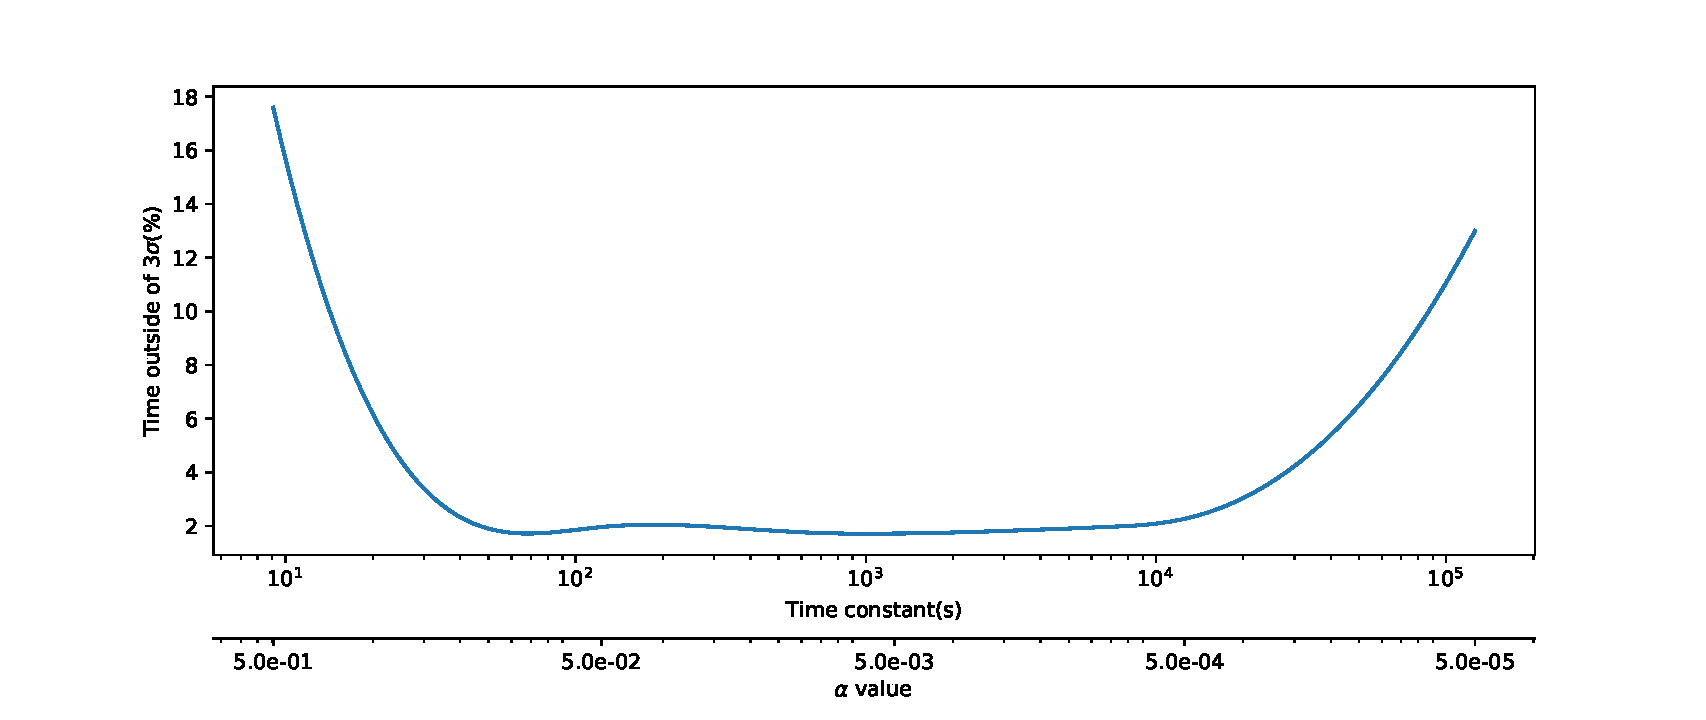
\includegraphics[width=1\linewidth]{img/napali_eval/a_selection.pdf}
    \caption{Amount of time a metric spends outside of the $3\sigma$ for various values of $\alpha$}
    \label{fig:expdes:6}
\end{figure}

The effect of the of selecting alpha as shown in Equation \ref{eq:opq_alpha} can be observed in Figure \ref{fig:expdes:7}.
This figure shows interesting features form the same dataset that was used to produce Figure \ref{fig:expdes:6}.
Blue traces show metrics that exhibit anomalous behaviour, while red indicates that Napali has flagged this temporal region as a sub-threshold event candidate.
Figure \ref{fig:expdes:7:1} shows a frequency fluctuation which nearly passes the threshold of $60.1Hz$ which would mark it as a full fledged event.
Instead, Napali marked almost the entirety of the fluctuation as a potential sub-threshold event, as shown by the red trace.
Figure \ref{fig:expdes:7:2} shows a step in the total harmonic distortion metric, similar to the one shown in Figure \ref{fig:opq:7} at the 6am mark.
In this case the metric in question abruptly changed to a new mean, requiring a fairly slow $\alpha$ coefficient to catch up over 3 minutes.
While it may seem wasteful to mark large temporal regions following an abrupt jump as candidates for sub-threshold event, it is important to note that:
\begin{enumerate}
    \item Making the $\alpha$ parameter smaller does not benefit the false positive rate as shown in Figure \ref{fig:expdes:6}.
    \item In-situ there is no way to tell if an abrupt shift is a switch to a new steady state, or if the metric will recover to a previous mean.
\end{enumerate}
It is important to remember than Napali is not meant to have a low false positive rate.
Instead, a system like OPQ Mauka can use all available information, including the raw data, to determine if an event is true gridwide event with much higher confidence.
The main goal of Napali is to have an extremely low rate of false negatives.
Figure \ref{fig:expdes:7:3} is on a different timescale from Figures \ref{fig:expdes:7:2} and \ref{fig:expdes:7:1}.
This is done in order to include several potential sub-threshold events into a common chart.
Five temporal regions during the the 3 Hrs are marked by Napali as potential sub-threshold events.
\begin{figure}[h]
    \centering
    \begin{subfigure}{0.5\textwidth}
        \centering
        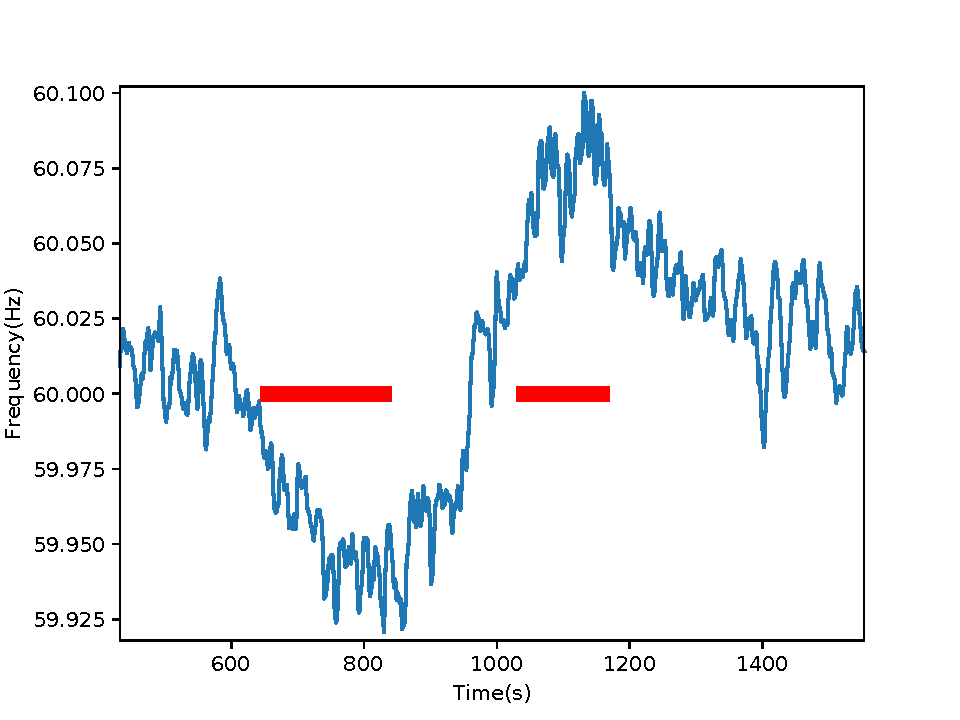
\includegraphics[width=1\linewidth]{img/napali_eval/napali_live_f.pdf}
        \caption{}
        \label{fig:expdes:7:1}
    \end{subfigure}%
    \begin{subfigure}{0.5\textwidth}
        \centering
        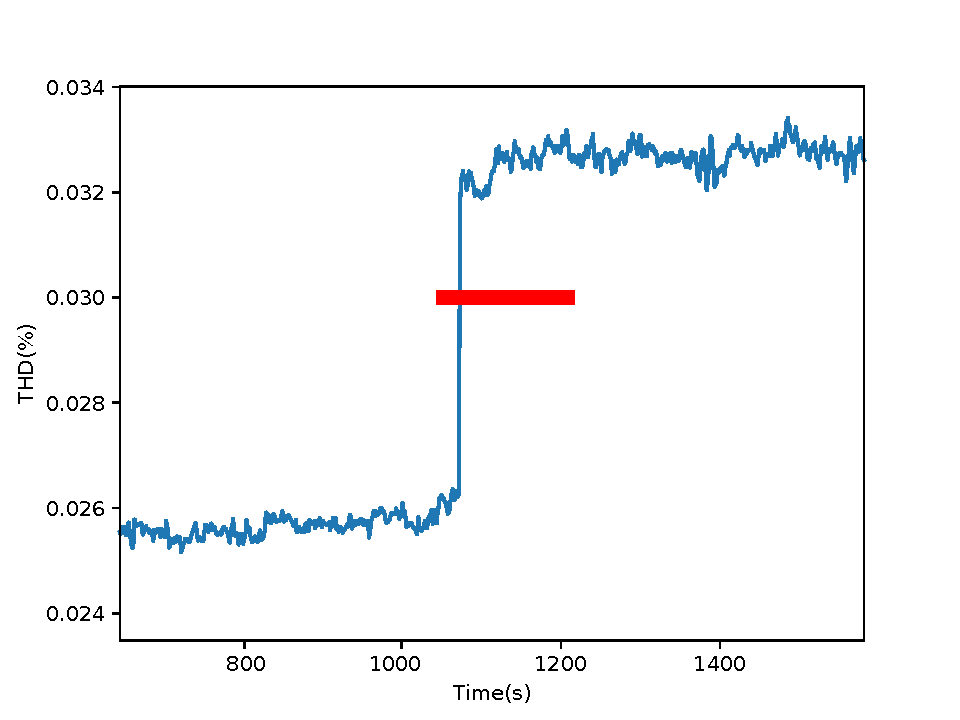
\includegraphics[width=1\linewidth]{img/napali_eval/napali_live_thd.pdf}
        \caption{}
        \label{fig:expdes:7:2}
    \end{subfigure}

    \begin{subfigure}{0.5\textwidth}
        \centering
        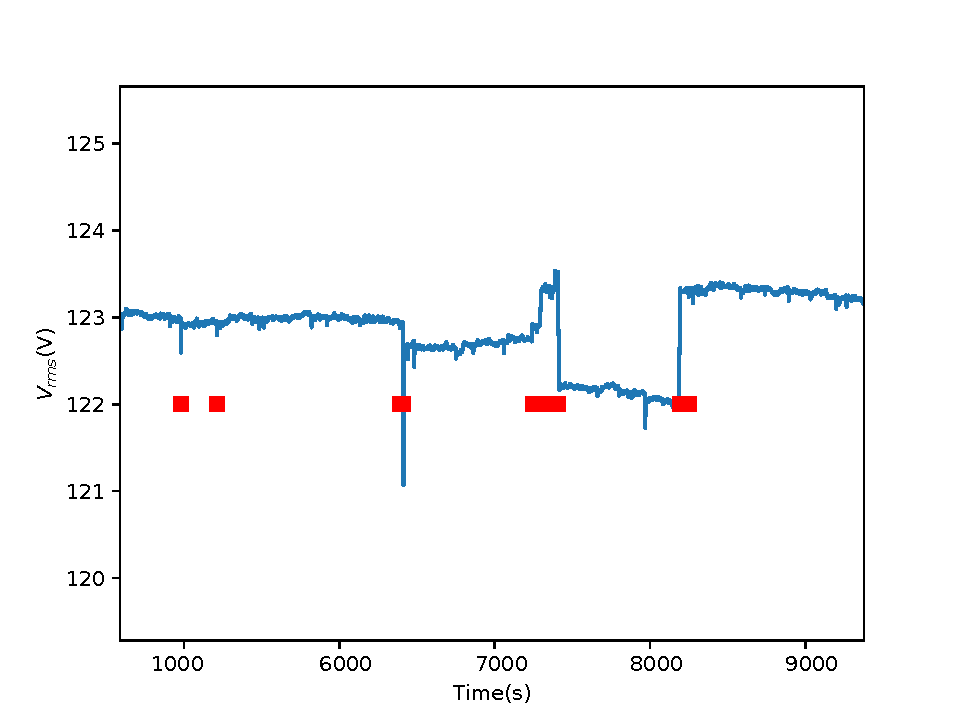
\includegraphics[width=1\linewidth]{img/napali_eval/napali_live_rms.pdf}
        \caption{}
        \label{fig:expdes:7:3}
    \end{subfigure}%
    \begin{subfigure}{0.5\textwidth}
        \centering
        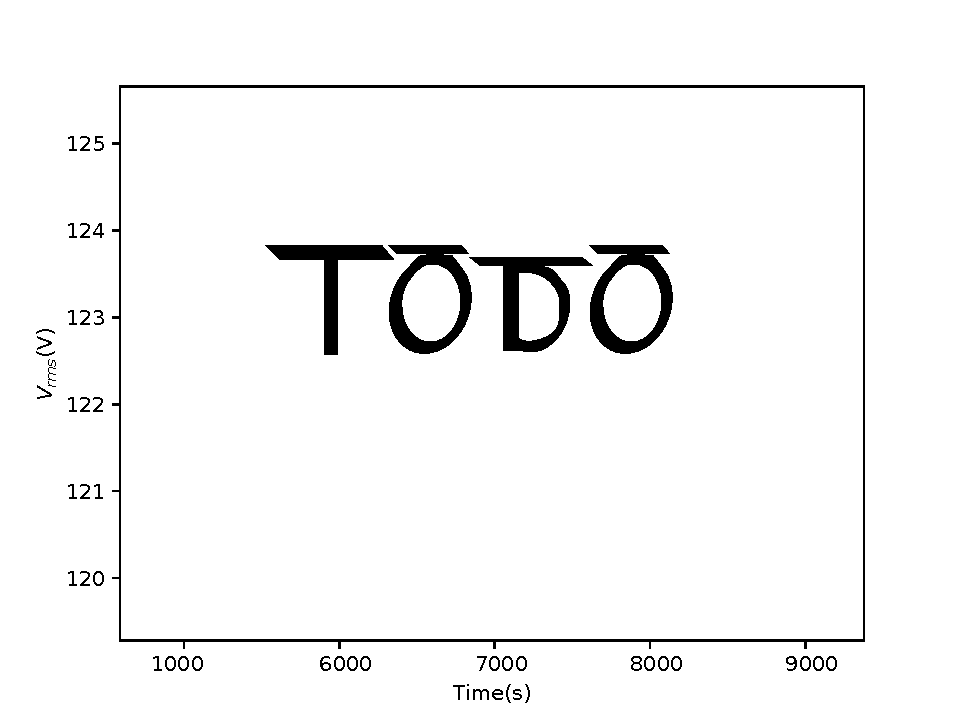
\includegraphics[width=1\linewidth]{img/napali_eval/napali_live_trans.pdf}
        \caption{}
        \label{fig:expdes:7:4}
    \end{subfigure}

    \caption{Potential sub-threshold events for a) $f_{fundamental}$, b)$THD$, c)$V_{rms}$ and d)$Trans$.
    Red boxes indicate that Napali picked these temporal windows as a potential sub-threshold event.}
    \label{fig:expdes:7}
\end{figure}

\subsection{Sub-Threshold Event Detection}\label{subsec:sub-threshold-event-detection}

One of the main goals of Napali is to utilize metric extraction in order to detect sub-threshold events.
During the deployment, two types of subthreshold events have been identified:
\begin{itemize}
    \item Partial sub-threshold event.
    \item Full sub-threshold event.
\end{itemize}
Full sub-threshold events consist of one or several devices passing the threshold described in Table \ref{tbl:opq:thresholds},
as well as one or several devices marked as sub-threshold by Napali.
Partial sub-threshold events consist of devices which all passed the threshold described in Table \ref{tbl:opq:thresholds}, however some of the devices triggered on a different metric with a much shorter temporal window.
The important distinction between partial sub-threshold events and regular events is that if triggered using the self-triggering method, the majority of the sub-threshold data would be lost.

\begin{figure}[h]
    \centering
    \begin{subfigure}{1\textwidth}
        \centering
        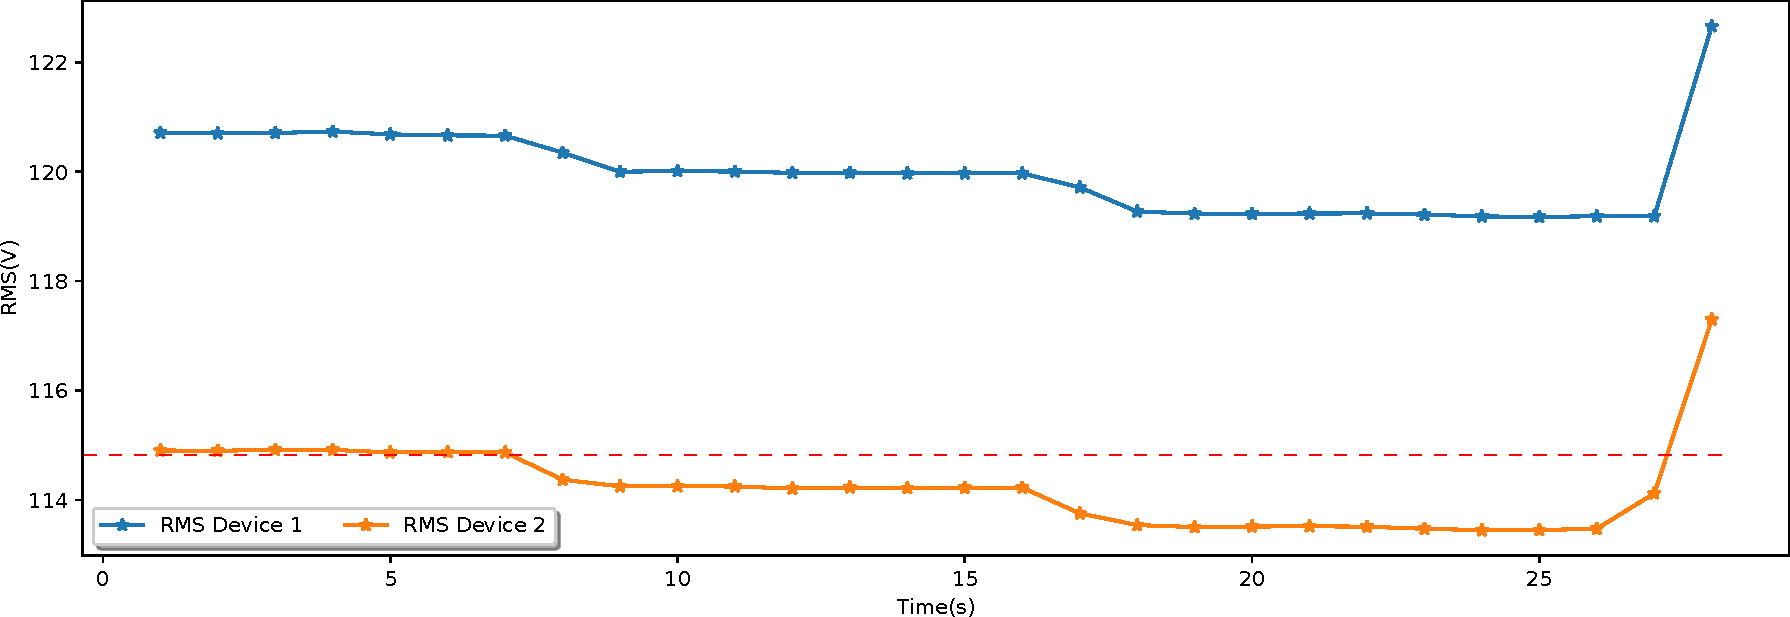
\includegraphics[width=1\linewidth]{img/napali_eval/rms_gridwide_subthreshold.pdf}
        \caption{}
        \label{fig:expdes:8:1}
    \end{subfigure}%

    \begin{subfigure}{1\textwidth}
        \centering
        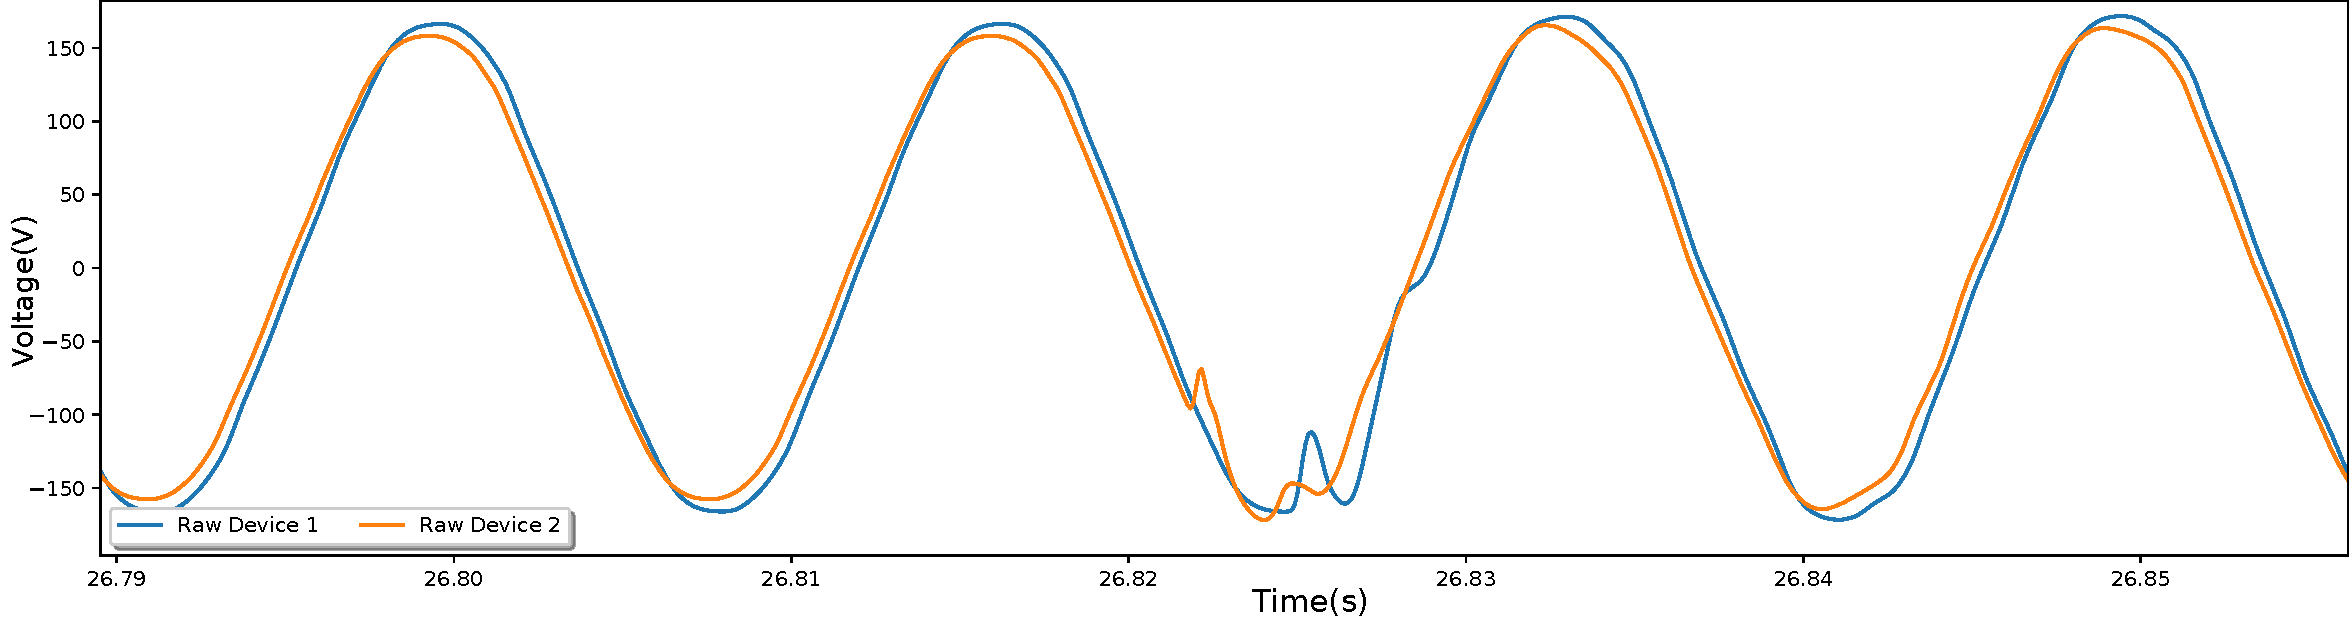
\includegraphics[width=1\linewidth]{img/napali_eval/raw_gridwide_subthreshold_zoom.pdf}
        \caption{}
        \label{fig:expdes:8:2}
    \end{subfigure}
    \caption{Partial sub-threshold event a) the sub-threshold component of the event, b) above threshold component of the event}
    \label{fig:expdes:8}
\end{figure}

An example of a partial sub-threshold event is shown in Figure \ref{fig:expdes:8}.
Figure \ref{fig:expdes:8:1} shows the sub-threshold component of the event.
In this event device 2 passed the threshold on $V_{rms}$ metric, initiating Napali to look for sub-threshold events across other devices.
It is important to note, that at the event start device 1 was considered to be a sub-threshold candidate, however, at $t \approx 26.8s$ device 1 produced a transient metric which was above napali threshold.
As such Napali requested raw data from both device 1 and device 2, creating a partial sub-threshold event containing both a voltage sag shown in Figure \ref{fig:expdes:8:1} and a transient shown in Figure \ref{fig:expdes:8:2}.

\begin{figure}[h]
    \centering
    \begin{subfigure}{0.49\textwidth}
        \centering
        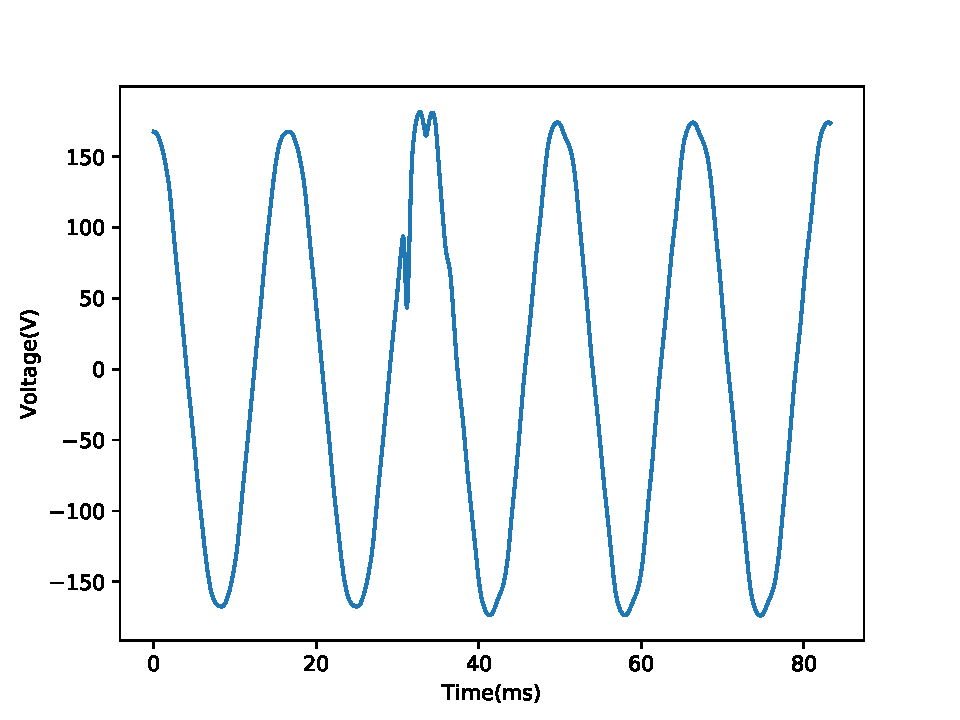
\includegraphics[width=1\linewidth]{img/napali_eval/raw_gridwide_sub_full1.pdf}
        \caption{}
        \label{fig:expdes:9:1}
    \end{subfigure}%
    \begin{subfigure}{0.49\textwidth}
        \centering
        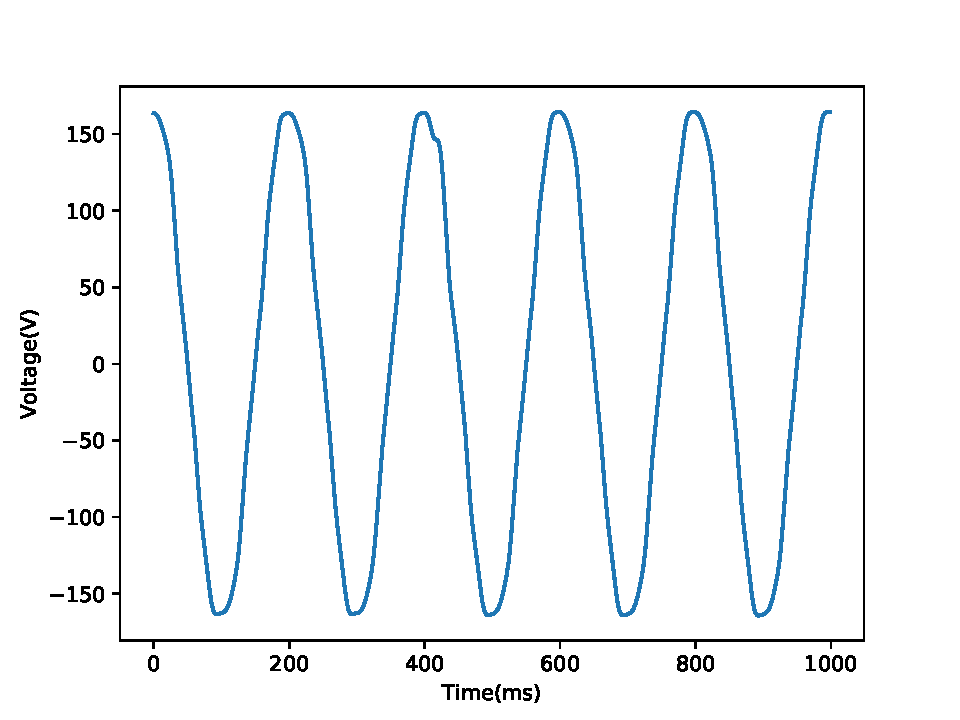
\includegraphics[width=1\linewidth]{img/napali_eval/raw_gridwide_sub_full2.pdf}
        \caption{}
        \label{fig:expdes:9:2}
    \end{subfigure}

    \begin{subfigure}{0.49\textwidth}
        \centering
        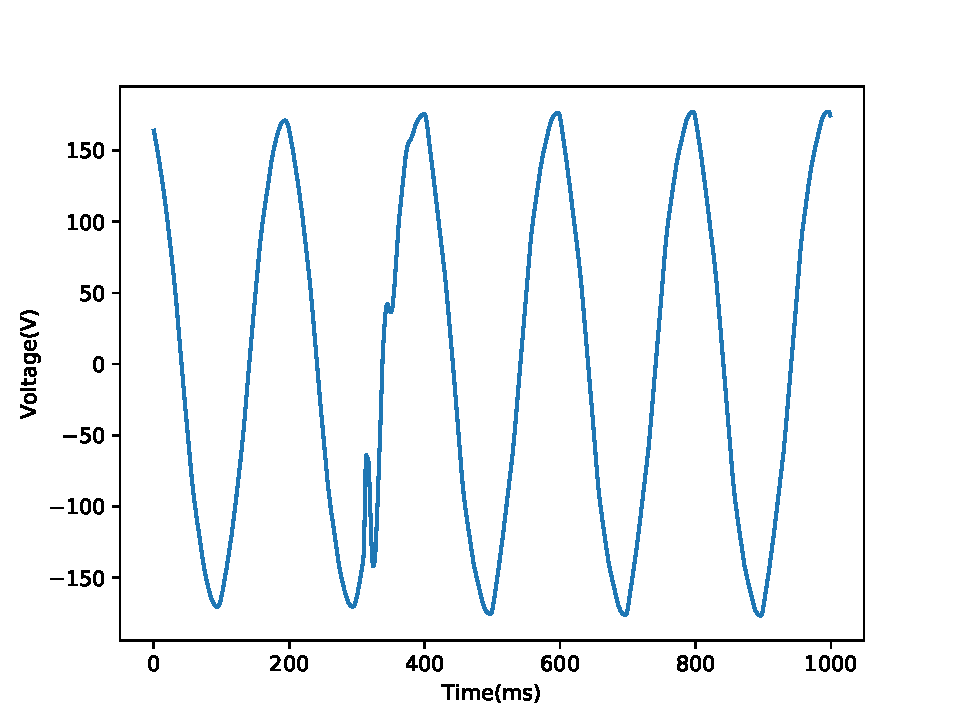
\includegraphics[width=1\linewidth]{img/napali_eval/raw_gridwide_sub_full3.pdf}
        \caption{}
        \label{fig:expdes:9:3}
    \end{subfigure}
    \begin{subfigure}{0.49\textwidth}
        \centering
        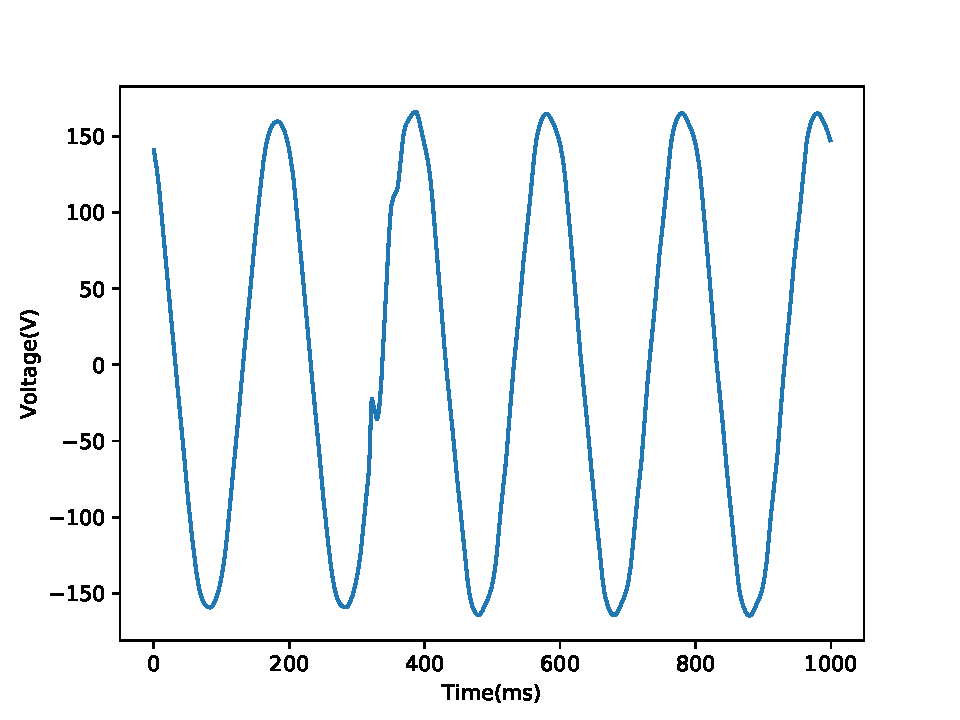
\includegraphics[width=1\linewidth]{img/napali_eval/raw_gridwide_sub_full4.pdf}
        \caption{}
        \label{fig:expdes:9:4}
    \end{subfigure}
    \caption{Full sub-threshold event across 4 devices.
    a) Device 1: above threshold b) Device 2: sub-threshold c) Device 3: above threshold d) Device 4: above threshold.}
    \label{fig:expdes:9}
\end{figure}

An example of a full sub-threshold event is shown in Figure \ref{fig:expdes:9}.
This is a short-lived transient event observed by four devices on September 5\textsuperscript{th}.
Devices 1, 3, and 4 generated a transient metric higher then the Napali threshold.
Device 2 transient metric did not pass threshold, yet nonetheless produced a severe enough deviation from the mean for Napali to consider it a part of the event.
This is particularly evident in the mild transient observed in Figure \ref{fig:expdes:9:2}.

\section{University of Hawaii Deployment.}\label{sec:university-of-hawaii-deployment.}

As part of the Napali validation, the OPQ system was deployed across the University of Hawaii Manoa campus (UH).
This location was ideal because it is an isolated microgrid connected to the Oahu powergrid only via a single 46kV feeder as shown in Figure~\ref{expdes:fig:1}.
Another advantage of the UH campus is the high number of smart meters deployed across various levels of the power delivery infrastructure.
While the purpose of these meters is monitoring the power consumption, they do include some rudimentary power quality monitoring capabilities.
Data from the campus deployed meters was used as ground truth for comparison against the measurements, and analysis performed by the OPQ project.
The location of smart meters in the grid topology is shown in figure~\ref{expdes:fig:1} as the $M$ nodes.
As evident by the meter location none of them were monitoring the consumer level power and mainly focused on the higher voltage power delivery.
This placement was a consequence of the smart meters role as a consumption monitor, and thus the deployment of the OPQ Boxes at the residential level complimented UH power quality monitoring capabilities without introducing redundancies.
University of Hawaii power grid is supplying a highly diverse infrastructure.
Beyond the traditional residential equipment such as computers and consumer grade electronics, the UH power grid powers scientific and laboratory equipment, machine shops, and server farms.
All of these elements have varying requirements/tolerances for power quality anomalies as well as different levels of power quality ``pollution''.
Furthermore, some of the electricity consumers in the UH campus are entirely unique.
For example, the free electron laser located in the Watanabe Hall is one of the only free electron lasers in the world, and the impact/sensitivity of power quality on the instrument are completely unstudied.
\begin{figure}[h]
    \centering
    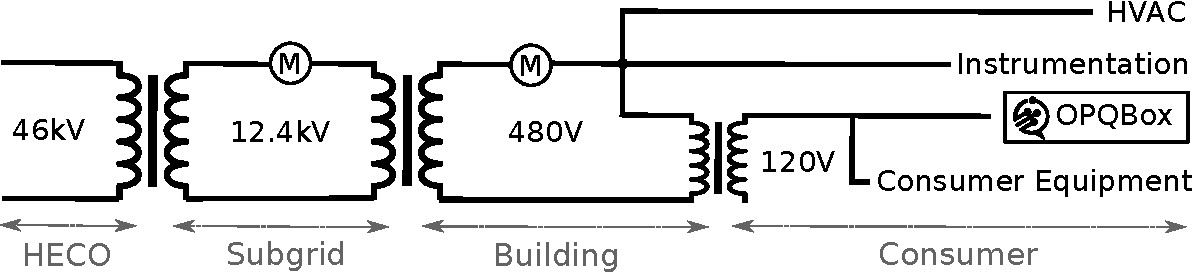
\includegraphics[width=1\linewidth]{img/uh-grid.pdf}
    \caption{University of Hawaii at Manoa power delivery infrastructure.}
    \label{expdes:fig:1}
\end{figure}

There were 74 smart meters deployed across the UH campus.
These meters measured the fundamental frequency $V_{rms}$, power consumption, reactive power, and power factor.
Data from these meters was cross-referenced with the Napali detection system in order to ascertain it's benefits.

OPQ Box placement was specifically selected to cover as much of the University of Hawaii power delivery infrastructure as possible.
The OPQ Box deployment is shown in Figure \ref{expdes:fig:deploy}.
By spreading out devices across the entire power grid, OPQ system is able to monitor the propagation of power quality disturbances throughout the UH power grid.
Consider the event shown in Figure \ref{fig:expdes:9}.
Figure \ref{expdes:fig:grid_wide_filtered} shows the same event with the fundamental and harmonics suppressed using a notch filter bank.
Furthermore, the location annotation is added to indicate the device location.
The most affected devices were located at the Physical Plant and Hamilton Library, recording a $~60V_{pp}$ transient.
Incidentally, both of these devices are monitoring a subgrid rooted at transformer(MA4).
Another device recorded this event was located in Watanabe Hall.
This device recorded a $30V_{pp}$ transient, still above the threshold for detection.
This device was monitoring the the subgrid rooted at the transformer LA4.
The final device was located at the parking structure entirely across campus.
This device recorded a $15V_{pp}$ transient, about 1V below the required magnitude for the threhold based detection.
However, Napali was able to determine that the parking structure OPQ Box was affected by the disturbance, and requested the raw data regardless.

\begin{figure}[h]
    \centering
    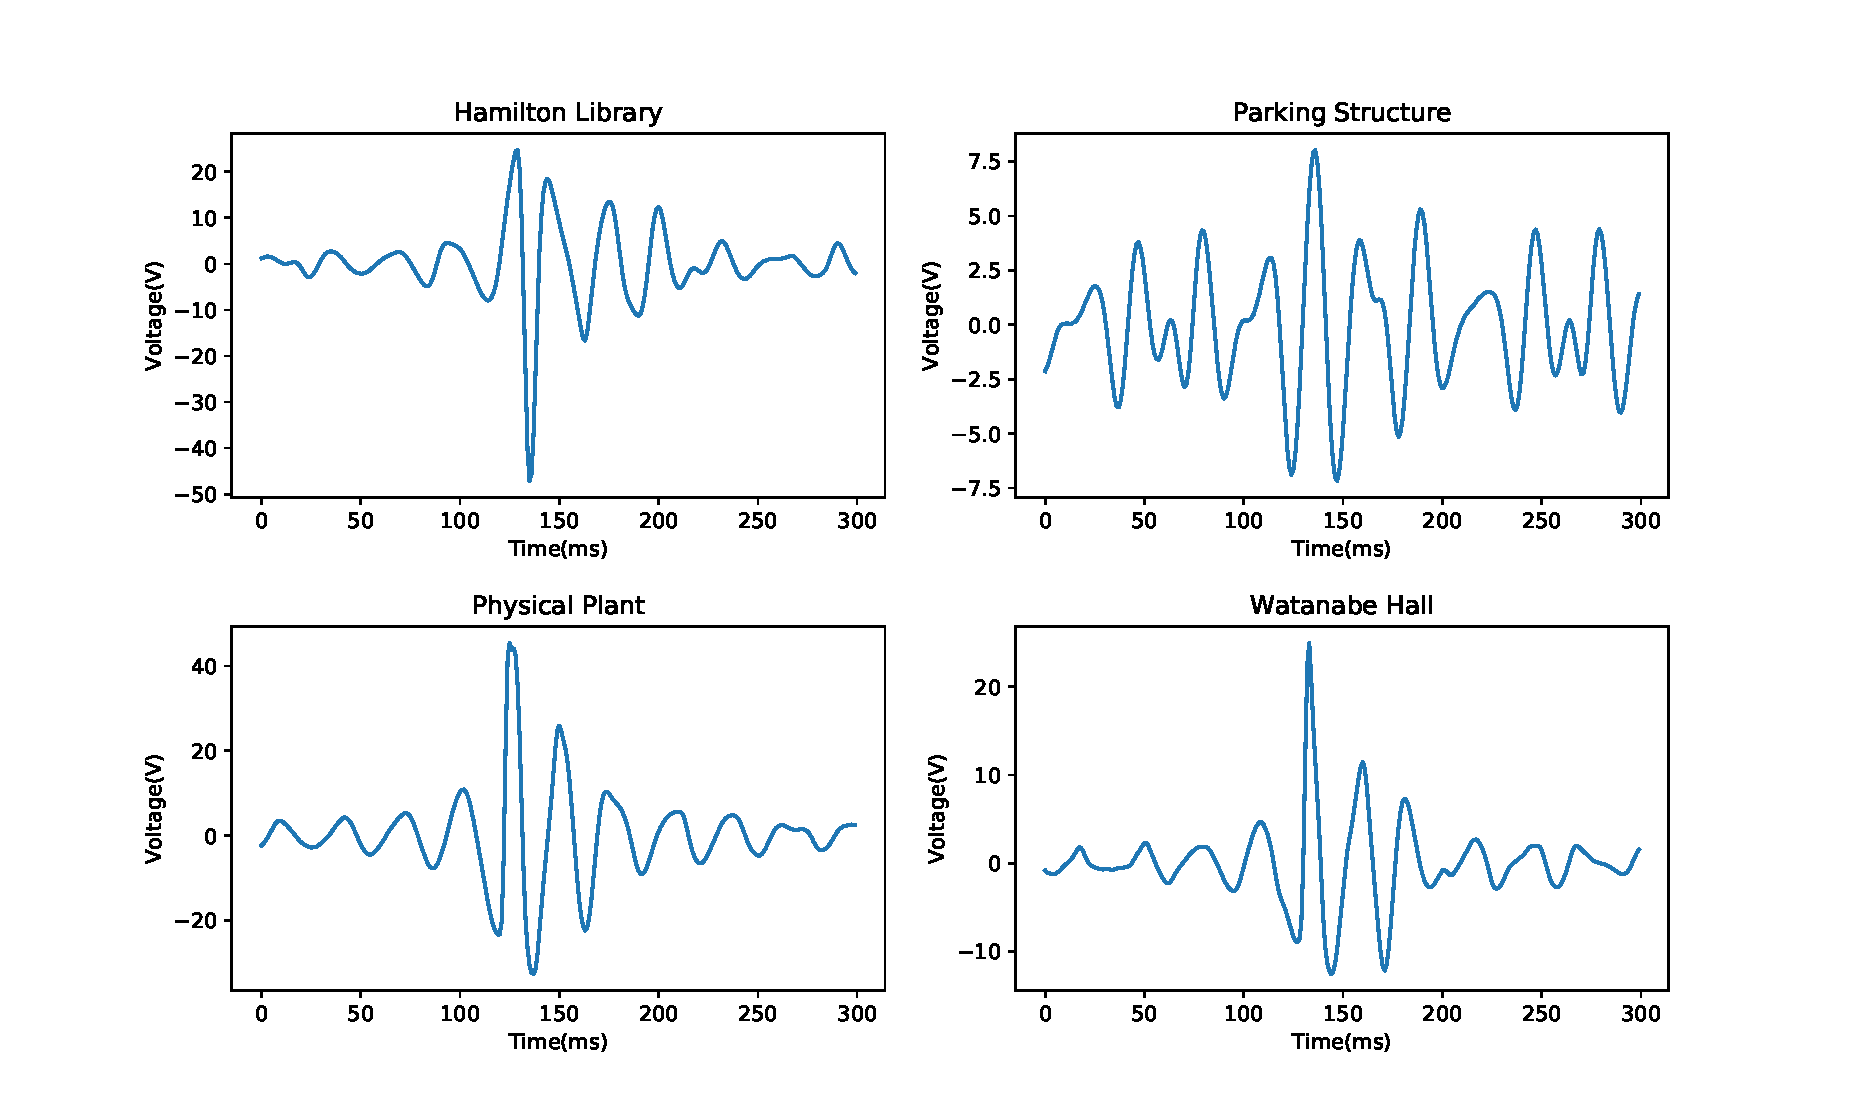
\includegraphics[width=1\linewidth]{img/deployment/gridwide_locality.pdf}
    \caption{Filtered Transient from event shown in Figure \ref{fig:expdes:9}}
    \label{expdes:fig:grid_wide_filtered}
\end{figure}

From the data gathered by Napali as shown in Figure \ref{expdes:fig:grid_wide_filtered}, it seems apparent that the disturbance originated at the subgrid rooted at the transformer MA4.
The Watanabe device was affected due to the short geographic and electrical distance to the MA4 subgrid.
By the time transient reached the parking structure, it was significantly attenuated by the transformers and transmission lines.
It was only detected due to the sub-threshold detection ability of the Napali framework.
\clearpage
\begin{figure}[h]
    \centering
    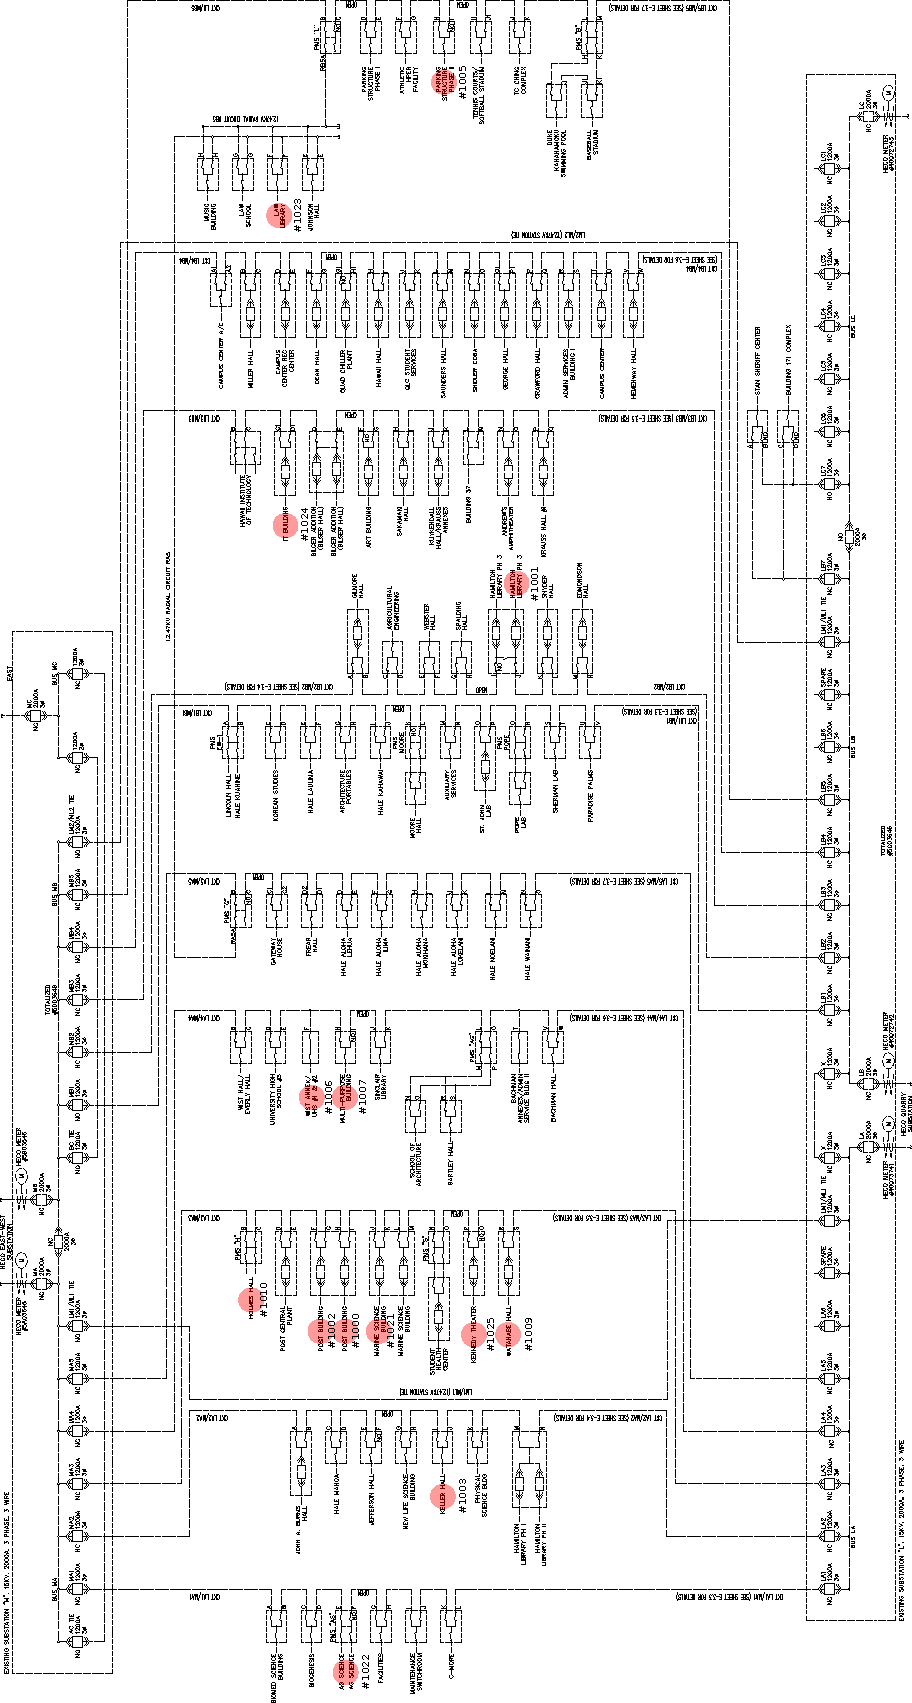
\includegraphics[width=0.7\linewidth]{img/deployment/uh_power_grid.pdf}
    \caption{OPQ Box locations and device IDs across University of Hawaii.}
    \label{expdes:fig:deploy}
\end{figure}

\clearpage

\subsection{Napali Bandwidth usage} \label{iexp:sec:band}
During the OPQ deployment It was found that Napali significantly outperformed both the self-triggered and the Naive event detection methods.
In order to evaluate the bandwidth performance of Napali a self-triggered plugin was ran along side it inside the Makai host.
This plugin utilized the same thresholds as Napali as described in Table \ref{tbl:opq:thresholds}.
However the self-triggered plugin did not take into the account any inter-device signatures.
This method is equivalent to each the device performing non-collaborative triggering.
\begin{figure}[h]
    \centering
    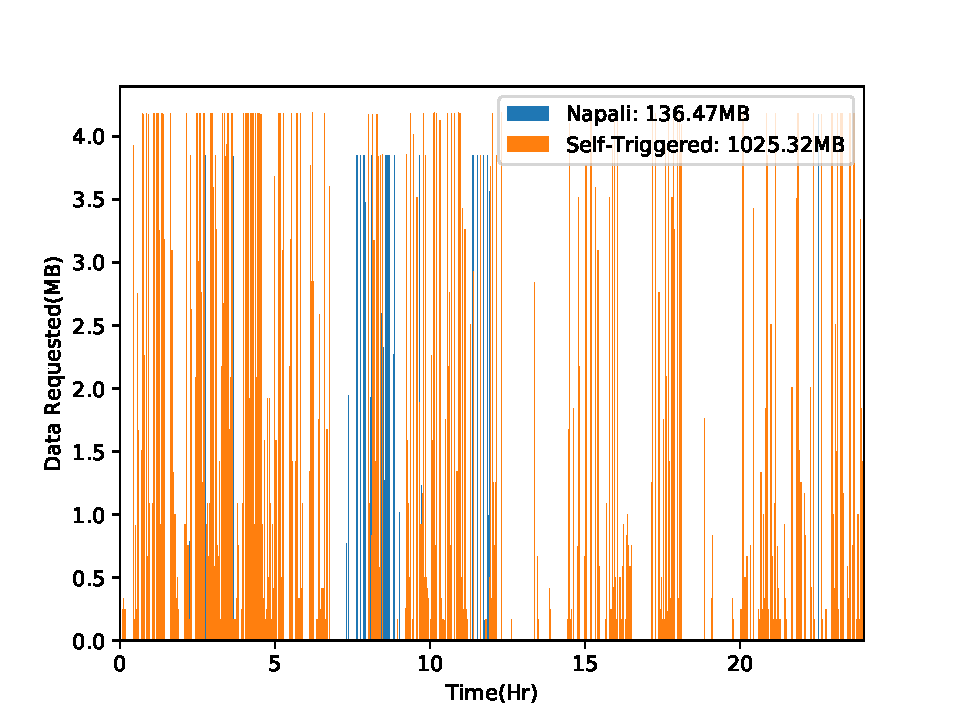
\includegraphics[width=0.8\linewidth]{img/napali_eval/napali_request_bandwidth.pdf}
    \caption{Amount of data requested from 10 OPQ Boxes via the self-triggered and Napali methods.}
    \label{expdes:fig:self_triggered_bandwidth}
\end{figure}

Figure \ref{expdes:fig:self_triggered_bandwidth} shows the amount of data requested from 10 devices by the self-triggered and Napali plugins over 24 Hours.
It is evident, that the majority of data requests for the self-triggered method resulted in local noise, and did not contribute to the grid measurements.
Napali on the other hand, ignored anomalies which did not affect more then a single device, while requesting sub-threshold data during a gridwide PQ event.

\begin{figure}[h]
    \centering
    \begin{subfigure}{.5\textwidth}
        \centering
        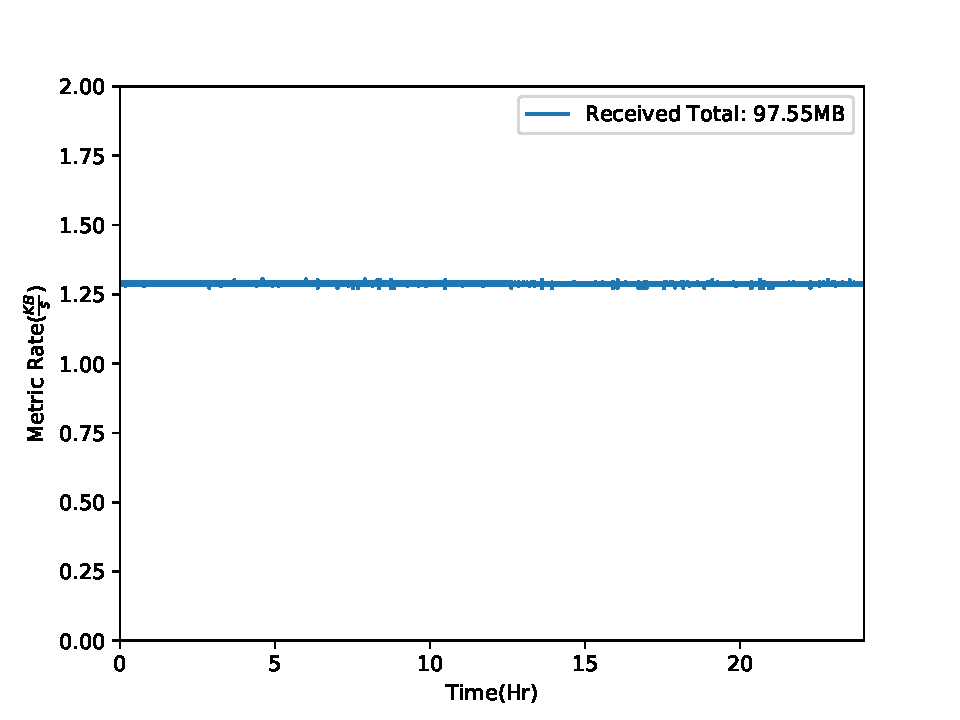
\includegraphics[width=1\linewidth]{img/napali_eval/napali_metric_bandwidth.pdf}
        \caption{}
        \label{expdes:fig:napali_metric_bandwidth}
    \end{subfigure}%
    \begin{subfigure}{.5\textwidth}
        \centering
        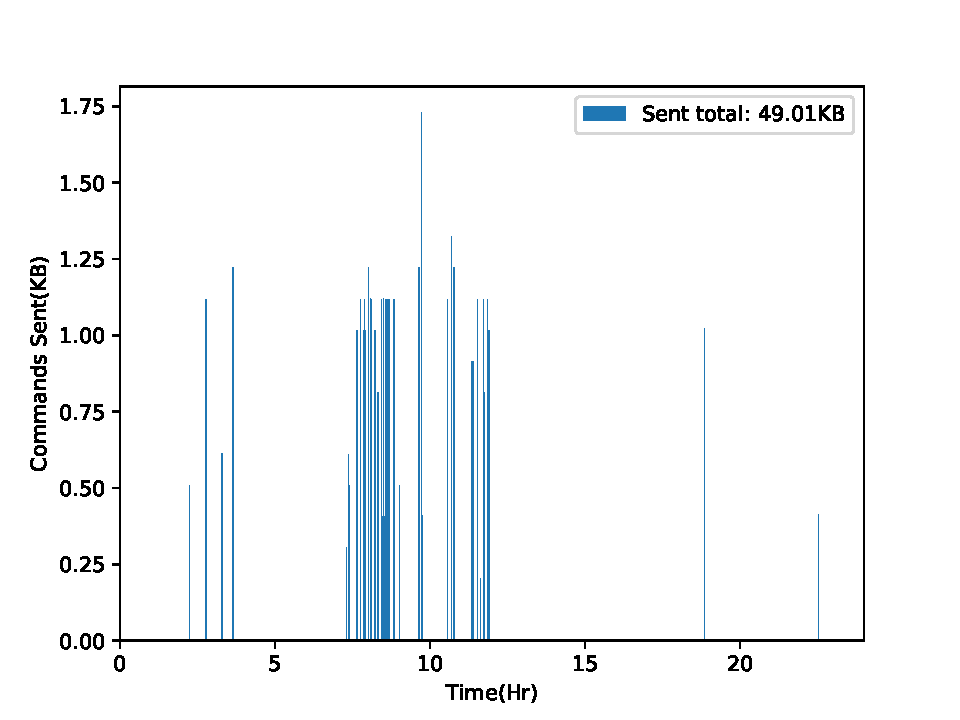
\includegraphics[width=1\linewidth]{img/napali_eval/napali_cmd_bandwidth.pdf}
        \caption{}
        \label{expdes:fig:napali_cmd_bandwidth}
    \end{subfigure}
    \caption{Penalties incurred by the Napali framework.
    a) Metrics received from 10 OPQ Boxes.
    b) Commands sent to 10 OPQ Box }
    \label{expdes:fig:napali_bandwidth_penalty}
\end{figure}

It should be noted that the self-triggered method does not incur the penalty of having to constantly transmit the device metrics to the sink, since all the event detection is performed on the device.
Figure \ref{expdes:fig:napali_metric_bandwidth} shows the amount of data received via metrics from 10 OPQ Boxes during the same 24 hours as the Figure \ref{expdes:fig:self_triggered_bandwidth}.
As expected the bandwidth requirement for metric transmission remains constant, since all OPQ Boxes send the metrics at fixed intervals.
While this penalty is significant as it constitutes 41\% of the total bandwidth used by Napali, the aggregate bandwidth is still shows a 440\% improvement over the self-triggered method.
Another penalty incurred by Napali is the two way communication requirement.
Each device which participated the event detection needed to receive a command with the temporal range which anomalous data.
Neither the naive nor self-triggered methods require two-way communication, and as such there is no direct comparison to Napali.
Figure \ref{expdes:fig:napali_cmd_bandwidth} shows the command bandwidth consumption for 10 OPQ Boxes across 24 hours.
The total consumption was ~50kB, which is quite trivial for any modern sensor network.

During the 24 hours of shown in Figures \ref{expdes:fig:napali_bandwidth_penalty} and \ref{expdes:fig:self_triggered_bandwidth}, Napali captured 60 events, while the self-triggered method captured 878.
The average length of the Napali Event was 10s to the self-triggered 3s.
Of 60 Napali events, all 60 contained sub-threshold data.

Comparison of Napali with the naive method was performed analytically.
Since the sampling rate of the OPQ Box is well characterized, and the number of OPQ Boxes is fixed, it is trivial to calculate the amount of raw data generated by the OPQ network during any time period.
In order to make this comparison fair, the raw data bandwidth will be scaled by the compression ratio of the state of the art compression algorithm specifically designed for power quality measurements.\cite{zhang2009new}
Operating at 12kSps, OPQ Box produces raw data at 24KB/s.
With state of the art compression operating at 90\% compression ratio and 5\% overhead of meta-data, one can expect a ~3KB/s stream of raw data for each OPQ box if it were to send the entirety of it to the sink.
For 10 OPQ Boxes we would expect the aggregate bandwidth of 30kB/s, and as such the bandwidth consumption 24.7GB/day.
During a 24 hour period, as shown in Figures \ref{expdes:fig:napali_bandwidth_penalty} and \ref{expdes:fig:self_triggered_bandwidth}, Napali used 234MB of bandwidth.
This corresponds to an over 100x improvement over the naive method.

\begin{figure}[h]
    \centering
    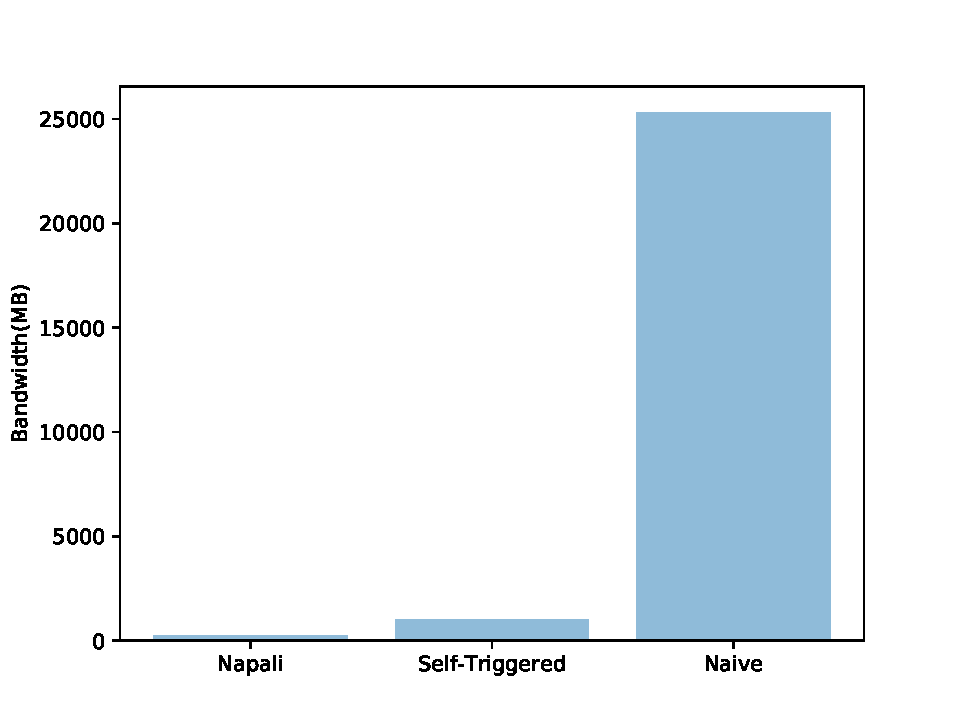
\includegraphics[width=0.8\linewidth]{img/napali_eval/napali_bandwidth_comparison.pdf}
    \caption{Bandwidth requirement comparison between three event detection methods.}
    \label{expdes:fig:bandwidth_master_comparison}
\end{figure}

Figure \ref{expdes:fig:bandwidth_master_comparison} shows the comparison between Napali as well as the naive and self-triggered methods.
While Napali incurs additional costs described in Figure \ref{expdes:fig:napali_bandwidth_penalty} it outperforms the comparable methods.
Finally, the cost of the two way communication as shown in Figure \ref{expdes:fig:napali_cmd_bandwidth} is greatly outweighed by the bandwidth savings in the raw data reception.
Modern sensor networks greatly benefit from two way communication, as it allows on-demand health monitoring, and software updates.
With addition of Napali, two way communication allows for significant bandwidth requirement reduction in for the sensor network as a whole.

\subsection{Sink processing requirement under the Napali Framework} \label{iexp:sec:scale}
Sink processing capacity between self-triggered, naive and Napali are quite different.
In general the processing requirement can be described as follows:
\begin{equation}\label{eq:detection_cost}
\begin{aligned}
    C_{total} = C_{metric} + C_{correlation}
\end{aligned}
\end{equation}
In the Equation \ref{eq:detection_cost} the $C_{total}$ is the total cost, $C_{metric}$ is the cost of extracting metrics, and $C_{correlation}$ is the cost of correlating metrics across device.
This stems from the fact that any event detection algorithm will first extract useful metrics from all devices on the network and then correlate these metrics to detect anomalies.

First, lets consider the Naive method.
In this case all of the metrics need to be extracted at the sync.
Disregarding the processing power required to keep up with the data rate described in Section \ref{iexp:sec:band} the metric processing cost can be measured imperially.
In order to do that the OPQ Box software was build for an x86 architecture and stress-tested.
Instead of acquiring data from a device driver, the feature extraction stack was supplied with synthetic data.
Finally the ZMQ communication was removed and replaced with the performance analysis code.
Stress test was performed on a Intel Core i9-8950HK CPU with thermal management disabled running at 2.9GHz.
Under such conditions, the metric extraction stack was able to extract features from 1s worth of raw data in $8ms$ running on a single core.
Since metric extraction has no inter-device data dependencies, a modern 8 core CPU we can expect to be able to extract features from 100 devices.

Self triggered method cuts down the amount of raw data that will be processed from each individual device by a factor of 25.
This means that metric extraction step computational resource consumption is reduced by the same factor.
Self triggered method can support up 2500 devices on a modern 8 core CPU.

Finally, Napali further reduces the metric extraction cost by filtering out local noise from the gridwide events.
A further 440\% efficiency from data size reduction results in a scalability improvements of 10000\% over the naive method.
As such a single 8 core CPU can support metric extraction for 10000 devices.
This can allow a single server running metric extraction to provide 5\% coverage of households in the city of Honolulu.
It is important to consider, that Napali already posses low fidelity metrics for every event it collects.
This in turn can also improve the scalability of Napali.
For example a common fundamental frequency extraction involves fitting a sine wave to the voltage waveform.
By using the coarse metric transmitted by the device, the fitter has a better initial condition, and thus will converge faster.



\subsection{Effects of latency in the Napali framework} \label{iexp:sec:lat}

\begin{figure}[h]
    \centering
    \begin{subfigure}{.45\textwidth}
        \centering
        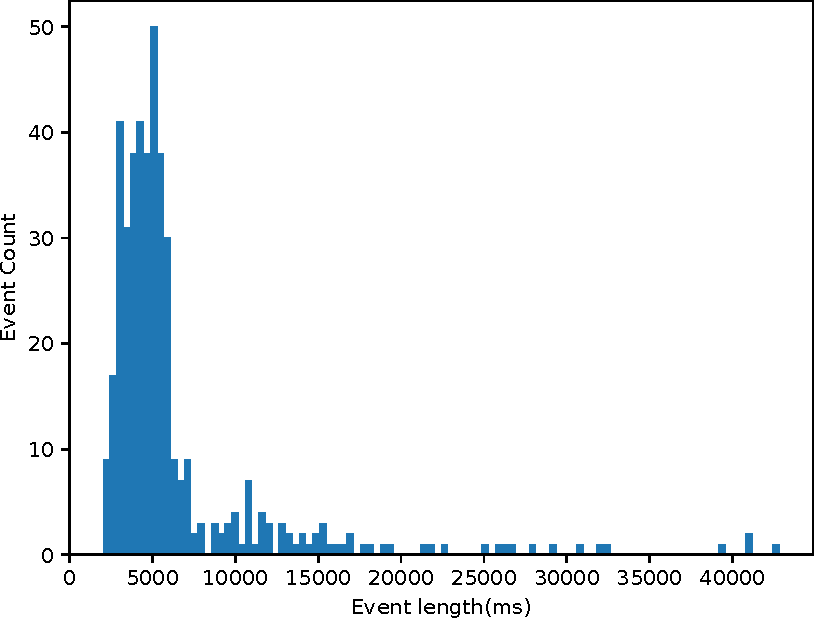
\includegraphics[width=1\linewidth]{img/napali_eval/event_length.pdf}
        \caption{}
        \label{expdes:fig:event_length}
    \end{subfigure}%
    \begin{subfigure}{.45\textwidth}
        \centering
        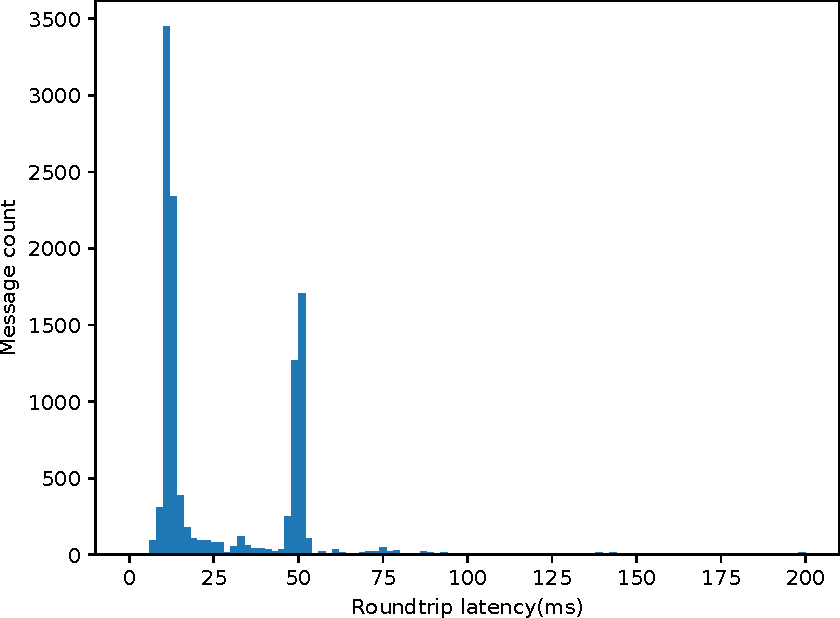
\includegraphics[width=1\linewidth]{img/napali_eval/latency.pdf}
        \caption{}
        \label{expdes:fig:latency}
    \end{subfigure}
    \caption{Event length(a) and message latency(b) observed by the OPQ devices.}

    \label{expdes:fig:el_la}
\end{figure}


The latency of Napali triggering system has a significant impact on its ability to read out complete raw data events.
Using generated distributed events as a baseline, I will be able to tune the threshold and temporal requirements for Makai detection algorithms.
Furthermore, temporal, spacial, and amplitude noise will be injected into the generated datasets, to simulate various uncertainties with regards to data collection, such as local noise, and NTP offset errors.
Taking into the account the detection latency of Makai, if some of the requested data is no longer available on the OPQ Box, only a partial time window will be returned.
These events will be marked as incomplete and their fraction as compared to the total number of events recorded will be used to establish the latency tolerance of the Napali framework.
Synthetic benchmarks will be carried out to establish the latency that the Napali system can incur without losing a portion of the event.
Since this is highly dependent on the amount of storage allocated for the RDRB, these experiments will be carried out with various RDRB settings.

Because OPQ Boxes operate using public University of Hawaii WIFI, the latency figures for data transmission are expected to be very dynamic.
In situations with large network contention, greater then 100ms one way packet latency can be expected.
This latency is exacerbated since at least three separate communication steps are required before raw data is received by Makai.
First the metric has to be sent to Makai, next if Makai detects an event, a data request needs to be sent to the affected boxes.
Finally boxes will forward raw data to the Makai sink.
I expect that with RDRB capacity of storing 5 seconds of raw data, no raw data events of 1s or shorter will be missed.
This figure allows for 1 second of transfer latency, 3 seconds of Makai analysis latency, and leaves 1 second of data in RDRB for readout.
However, these figures can only be validated in a real world situations.

\subsection{Temporal locality triggering of the Napali framework} \label{iexp:sec:loc}
Once the OPQ Box is fully validated and the Makai detection thresholds are tuned using synthetic datasets, the Napali system will be fully deployed at the University of Hawaii at Manoa.
 Every time the Napali detects an event, both OPQ Boxes and building meters will be queried for data.
 While it may be unfeasible to query raw data from the UH metering infrastructure, metrics are readily available.
 This data will be used to ascertain the proportion of false positive events detected by Napali.
 Additionally, the internal single point fault detection mechanism of the UH power meters will be used in conjunction with the events detected by Napali to measure the rate of false negative events.
 Both the false negative and false positive measurements will be used to ascertain the detection efficient of the Napali framework.
 This analysis will also include an evaluation  of Napali's ability to reject single point anomalies.
 For a portion of OPQ deployment, every event triggered by a single device will be captured.
 These events will be analyzed in order to determine if a gridwide anomaly was incorrectly classified as a single point disturbance.

The goal of Napali is not to to provide a zero false positive rate.
Once raw data is stored, higher level processing can further filter and classify it using more computationally expensive techniques.
As long as the bandwidth consumption of Napali compares favorably to sending the entirety of raw data to the sink, any rate of false positives can be tolerated.
False negatives on the other hand are the primary metric subject to optimization.
Ideally a zero rate of false positives would be expected, however as with any real-world system I do not expect that to be the case.
This evaluation will determine the triggering efficiency of the Napali framework when compared to the detection ability of a commercially available system.

\subsection{Sub-threshold Data Acquisition} \label{iexp:sec:sub}
The Napali methodology will be compared with the single point anomaly detection approach.
In order to do that I will compare the extent to which sub-threshold events are missed by the UH metering infrastructure.
In a large distributed event, if a portion of events are not detected by the UH meter's single point detection, but picked up by the Napali framework, these events will be flagged and analyzed for their merit.
This will in turn provide a metric of distributed detection ability of the Napali framework compared to commercial system.
Furthermore, for a portion of the deployment the triggering stream from the OPQ Boxes will be stored along with the acquired raw data.
The triggering stream can be used to compute which fraction of devices would have self triggered if operating autonomously.
This will provide the baseline for sub-threshold triggering efficiency of the Napali system, with respect to the single point detection ability of the OPQ Box.

This evaluation will compare Napali performance to the single point detection mechanisms currently in deployment.
I expect that Napali will outperform these strategies, and provide a more complete picture of gridwide anomalies as they propagate through the UH power grid.
It is possible that no sub-threshold events will be recorded during the UH deployment.
UH campus is quite small, perhaps too small for an anomaly in one building not to impact the rest of campus.
In this case the sub-threshold data acquisition will remain an open topic for future work and a larger geographical deployment.
Regardless, as long as I am be able to validate the single point anomaly rejection ability of Napali as described in Section~\ref{iexp:sec:loc}, I will be able to conclude that Napali has a distinct advantage over single point detection methods.
Single point anomalies are not important in smart grid monitoring, since they originate from the consumers side of the meter, and should be ignored.
In fact, recording these events may be detrimental to the privacy of the end-user, since it may give clues on their activities as shown in Figure~\ref{intro:fig:1} a and b.
However since privacy implication of power quality monitoring are outside the scope of this project, this study will remain as a point of future work.
